\chapter{Úvod}
\blind{3}

\chapter{Neformální návrh systému} \label{section:draft}
Cílem této práce práce je vytvořit systém pro strojový překlad textu pomocí umělých neuronových sítí. Pro snadnou představu, je to totéž jako to co dělá Google Translator\footnote{translate.google.cz} blíže popsáno v článku \cite{googleBridgingGap}. Vezme se věta v původním jazyce a vytvoří se z ní co nejvěrnější překlad v jazyce cílovém a to za pomocí nacvičené neuronové sítě. V této kapitole je vysvětleno jak by takový systém mohl vypadat a co za komponenty potřebuje k tomu aby fungoval.

\begin{description}
  \item[Dataset] aby bylo možné něco překládat, je nejprve zapotřebí mít nějaký dataset. Dataset obsahuje texty ve dvou jazycích mezi kterými se má překládat. Tyto texty musí být zarovnané, tak aby si jednotlivé věty v těchto jazycích navzájem odpovídaly. Obecně platí, že čím větší množství použitých dat a čím větší model, tím lepší bude výsledek.Použít nebo ne?\cite{googleLimits}
      \todo{v kapitole o implementaci pak dát zná zorňující obrázek}

  \item[Tokenizer] Dataset a jeho jednotlivé věty před začátkem trénování sitě je nejprve potřeba předpřipravit. Tokenizer rozdělí věty na jednotlivé tokeny \todo{obrázek ukázky tokenizace}. To usnadňuje práci s datasety a také například snižuje velikost slovníků (všech vyskytujících se slov/tokenů v datasetu pro jeden jazyk).
  
  \item[Slovník] Slovník se vytvoří jako seznam n nejčastějších slov v datasetu ve vstupním a cílovém jazyce. Čím je slovník menší, tím se zmenší výpočetní požadavky, ale na druhou stranu je potřeba vyřešit při trénování a překladu problém se slovy mimo slovník (OOV -- out of vocabulary). \todo{kde budou popsány unk symbol a tak..v implementaci?}
  
  \item[Word Embeddings] Obecně je možné vytvářet jazykové modely, které generují text po písmenech, částech slov nebo po slovech \url{http://www.fit.vutbr.cz/~imikolov/rnnlm/char.pdf}. V této práci se bude pracovat s celými slovy (tokeny). Word Embeddings je další forma předzpracování. Každý token ze vstupního slovníku se převede vektoru reálných čísel, ve kterém jsou zakódovány některé syntaktické a sémantické vlastnosti daného tokenu, což umožní neuronové síti se učit lépe, než kdyby se použilo například jenom číslo označující pozici tokenu ve slovníku. \todo{nějaká sekce o slovnících?} Více v sekci \ref{section:embeddings}.

  \item[Model] Pro překlad je nejvhodnějším modelem sequence to sequence (dále seq2seq \cite{seq2seq}) s použitím encoder-decoder architektury. Na rozdíl od starších statistických metod překladu, kde se překládalo po frázích, moderní překlad pomocí neuronových sítí probíhá po celých sekvencích (větách). Nejprve enkodér vezme word embedding na vstupu a pomocí rekurentní neuronové sítě\ref{section:rnn} převede větu na vstupu do velkého vektoru reprezentující její význam. Dekodér -- taky rekurentní neuronová síť -- následně z tohoto vektoru slovo po slovu vygeneruje výslednou přeloženou větu. Dekodér tedy funguje jako jazykový model \ref{section:langmodel}, který je na inicializovaný na jednu konkrétní větu.
\end{description}


\begin{figure}[h]
    \begin{center}
            \tmpframe{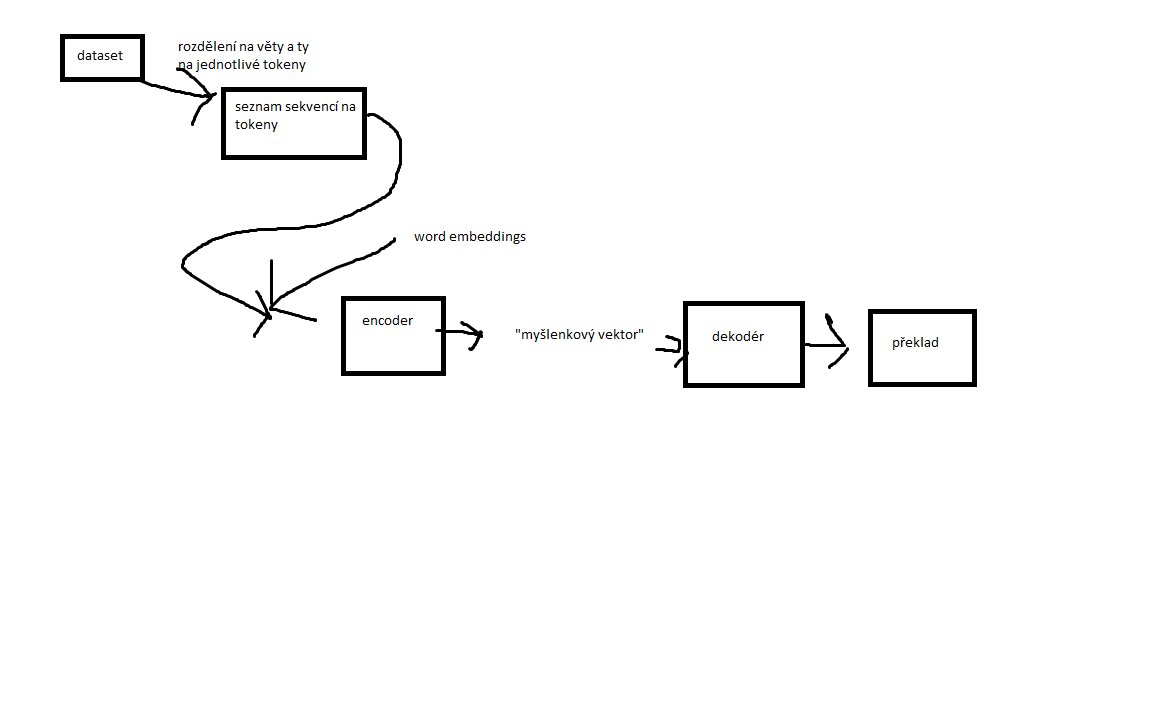
\includegraphics[width=1.0\linewidth]{img/draft.png}}
    \end{center}
	\caption{schéma návrhu systému pro překlad}
	\label{img:draft}
\end{figure}


\chapter{Související teorie a pojmy}
Účelem této kapitoly je blíže vysvětlit a rozebrat jednotlivé pojmy a komponenty potřebné pro vytvoření překladového systému. 



\section{Jazykové modely}\label{section:langmodel}
\todo{citace?}
Zatímco u programovacích jazyků existuje jejich formální definice, přesně popisující jejich syntaxy a význam, u přirozených jazyků to tak není. Přirozený jazyk vznikl náhodným způsobem v průběhu staletí a tisíciletí narozdíl od formálně definovaných jazyků, které byly přímo navrženy. Přestože běžný jazyk se řídí nějakými pravidly, existuje značné množství výjimek a odchylek. I napříč tomu si však lidé navzájem rozumí. Problém však je tyto pravidla převést do formálních pravidel, tak aby jim rozuměl počítač. Řešením pro tento problém mohou být jazykové modely, které nevznikají pomocí definice formálních pravidel, ale učením se z příkladů.

Jazykový model udává pro každou větu $w$ jaká je její pravděpodobnost. Respektive pro sekvenci slov $w = w_1, w_2..., w_m$ získá pravděpodobnost podle \ref{figure:probdistr}.

\begin{align}\label{figure:probdistr}
  p(w) = \prod_{i=1}^{m} p(w_i|w_{<i})
\end{align}

Pro každé slovo $w_i$ ze sekvence určí jaké je jeho podmíněná pravděpodobnost v případě, že se před ním nachází slova $w_i$.

Ve výsledku tak jazykový model umožní zhodnotit přirozenost věty a generovat text podobný tomu, na kterém byl model nacvičen \cite{nmtTutorial}.

\begin{description}
  \item[Zhodnocení přirozenosti] Pomocí jazykového modelu je možné pro větu $w$ zhodnotit, jak moc je přirozená nebo-li jak moc je pravděpodobné, že by takováto věta mohla existovat v textu na kterém byl model nacvičen.
  \item[Generování textu] Protože model umožňuje pro každé slovo $w_i$ získat pravděpodobnost následujícího slova $w_{i+1}$, je takto možné generovat náhodný, přirozeně (vůči zdrojovému textu) vypadající text. Což je přesně potřeba pro generování překladů.
\end{description}


\todo{jazykove modely v kontextu machine translation, generovani jazyku}



Handling Unknown Words \cite{nmtTutorial}

\subsection{N-gram}
\subsection{log-linear}


\subsection{Word embeddings}\label{section:embeddings}
\todo{souvislost s jazykovymy modely}

\todo{více v sekci ... .. a tam budou obrázky, rovnice, vysvětlení...}

\begin{figure}
    \begin{center}
            \tmpframe{
\includegraphics[width=0.5\linewidth]{img/placeholder.pdf}}
    \end{center}
	\caption{One image. \todo{Napsat pořádný titulek}}
	\label{img:TODO}
\end{figure}

Zmíním co existuje za druhy, lehce jejich rozdíly a vznik (co jsou zač) a pak se víc rozepíšu o fasttextu, protože to je ten co jsem použil (rovnice a kdesi cosi)
\begin{itemize}
  \item word2vec
  \item glove
  \item fasttext
\end{itemize}

\section{Rekurentní neuronové sítě}\label{section:rnn}
V této kapitole je popsán základní koncept rekurentních neuronových sítí (RNN\footnote{z anglického recurrent neural network}), jejich srovnání s běžnými neuronovými sítěmi a dále pak popis upravených variant RNN -- LSTM \ref{section:LSTM} a GRU \ref{section:GRU}. Sekce volně vychází z práce \cite{nmtThesis}.\\


RNN (Elman \cite{rnn}) jsou známé již přes dvě desítky let. Úspěšně jsou však používány až v posledních letech a to hlavně díky vyššímu výpočetnímu výkonu a většímu objemu trénovacích dat, který je v současné době dostupný a také, díky většímu výkonu, zpracovatelný. Tento druh neuronových sítí je obzvlášť vhodný například pro rozpoznávání psaného písma, rozpoznávání řeči, v kombinaci s konvolučními neuronovými sítěmi pro generování popisků obrázků a co je nejvíce zajímavé pro tuto práci, pro tvorbu jazykových modelů, generátorů textu a pro překlad.

Jejich hlavních výhodou oproti původním dopředným neuronovým sítím je jejich schopnost držet si vnitřní stav napříč časem. Dopředná neuronová síť pracuje vždy s aktuální hodnotou $x$ na vstupu, pro kterou pomocí vah $W$ získá výstup $y$ (rovnice \ref{figure:basic-nn}).

\begin{align}\label{figure:basic-nn}
  y = f (x, W)
\end{align}

Pokud pak takováto síť pracuje s nějakou sekvencí měnící se v čase, například se slovy v rámci jedné věty, pro každé slovo na vstupu $x_t$, kde $t$ znázorňuje čas (pozici) slova ve větě, použije stejné váhy pro získání výstupu $y_t$ a nezjistí ani nezachová žádnou úvahu o vzájemném vztahu těchto slov.

RNN tento problém řeší zavedením vnitřního stavu $h_t$ a smyčky (obrázek \ref{img:rnn-rolled}). Vstupem dalšího stavu je vždycky výstup ze stavu minulého. Pro každé $x_t$ ze sekvence se tedy nyní může získat výstup $y_t$ pomocí vnitřního stavu $h_t$ z předchozího kroku $t$ (rovnice \ref{figure:rnn}. Přičemž počáteční stav  $h_0$ je obvykle nastaven na nulu.

\begin{align}\label{figure:rnn}
  h_t = f (x_t, h_{t-1})
\end{align}

\begin{figure}[h]
    \begin{center}
            \tmpframe{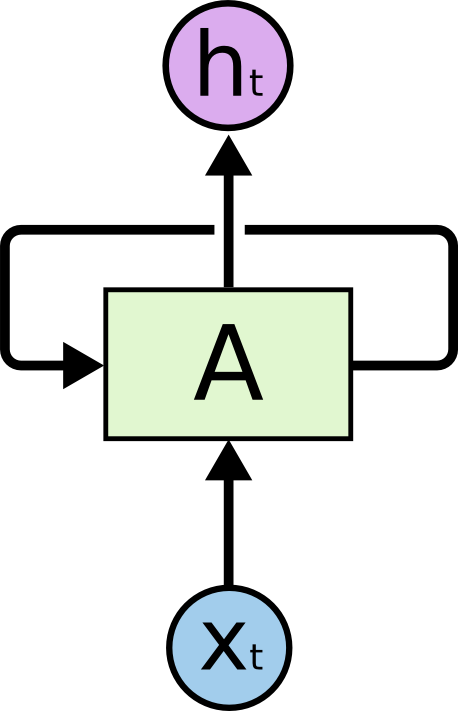
\includegraphics[width=0.3\linewidth]{img/RNN-rolled.png}}
    \end{center}
	\caption{Recurrent Neural Networks have loops. \todo{vlastni obrázek nebo citace \url{http://colah.github.io/posts/2015-08-Understanding-LSTMs/} }}
	\label{img:rnn-rolled}
\end{figure}

Funkce $f$ z rovnice \ref{figure:rnn} je nelineární funkcí a nejčastěji se používá jedna z funkcí \emph{sigmoid}, \emph{tanh} nebo \emph{relu} \ref{img:functions}. \todo{lepe popsat jednotlivé funkce a jejich výhody/nevýhody}

\begin{figure}[h]
    \begin{center}
            \tmpframe{
\includegraphics[width=0.3\linewidth]{img/placeholder.pdf}}
            \tmpframe{
\includegraphics[width=0.3\linewidth]{img/placeholder.pdf}}
            \tmpframe{
\includegraphics[width=0.3\linewidth]{img/placeholder.pdf}}
    \end{center}
	\caption{\todo{vedle sebe obrazky funkci relu, tanh, sigmoid, idealne tri ruzny captions}}
	\label{img:functions}
\end{figure}


\begin{align}\label{figure:softmax}
  \sigma (\mathbf {z} )_{j}={\frac {e^{z_{j}}}{\sum _{k=1}^{K}e^{z_{k}}}}
\end{align}


\begin{figure}[h]
    \begin{center}
            \tmpframe{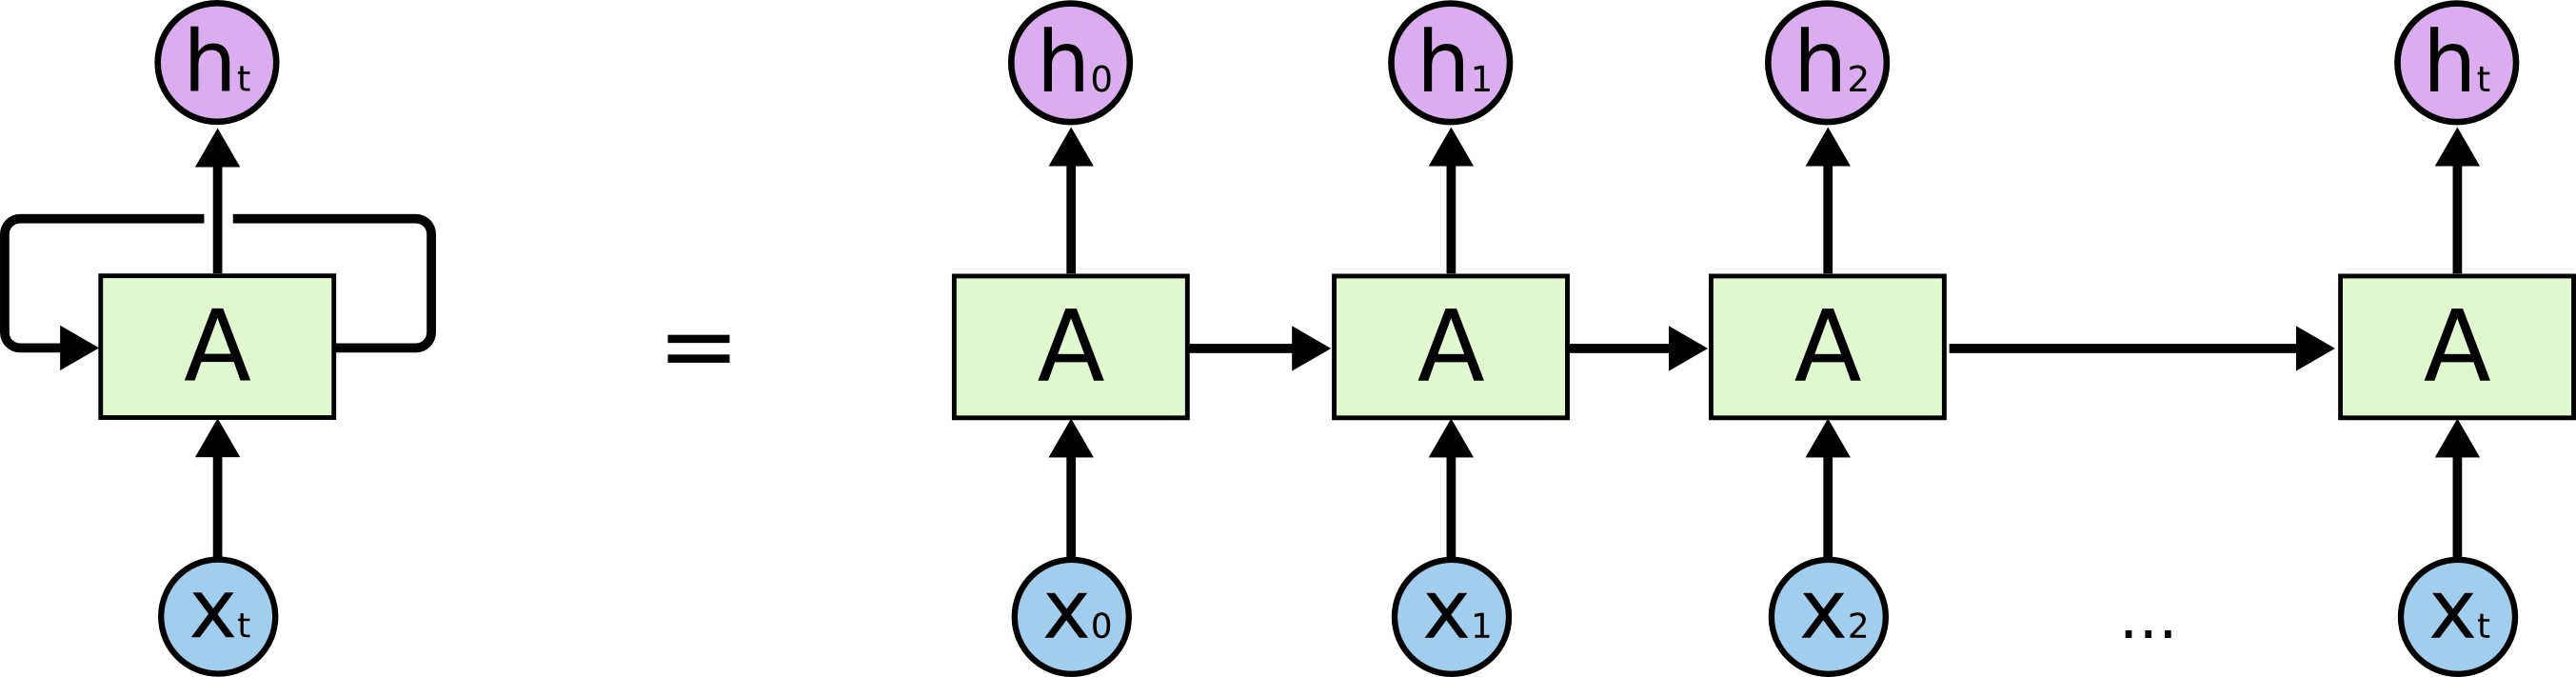
\includegraphics[width=1.0\linewidth]{img/RNN-unrolled.png}}
    \end{center}
	\caption{A recurrent neural network and the unfolding in time of the computation involved in its forward computation. \todo{vlastni obrázek nebo citace \url{http://colah.github.io/posts/2015-08-Understanding-LSTMs/} }}
	\label{img:rnn}
\end{figure}

\todo{doplnit rovnice a vysvětlení jak se to aplikuje dál, stejně tak obrázky s unrolled rnn a popisem toho jak zachovává nějakou informaci (třeba že podstatné jméno je mužské) skrze jednotlivé kroky (i když ne úplně přes vzdálené a tím se dostanu k long term dependencies)}


\todo{trénování rnn, back propagation through time, have difficulties (\url{http://proceedings.mlr.press/v28/pascanu13.pdf}) learning long term dependencies}
\todo{loss computing}
\todo{gradient computing}
\todo{související vanishing a exploding gradient problem popsáno v \cite{gradientProblems}, je to docela popsany i v nmtTutorial}
\todo{predchazeni vanish/exploding - lstm a gru, ktery s tim nejak pocitaji. Regularization - vysvětlit co to je}

\todo{zvlášť neuronky a to jakým způsobem se učí/optimlizují(gradient..) a pak až konkrétně rekurentní nebo rovnou rekurentní?}
\todo{deep, bi-directional}


\subsection{LSTM}\label{section:LSTM}
LSTM (Long short term memory \cite{LSTM} je varianta RNN řešící problém mizejícího gradientu a vzdálených závislostí \todo{lepší překlad pro long term dependencies?}.

\begin{align}
    f_{t}&=\sigma _{g}(W_{f}x_{t}+U_{f}h_{t-1}+b_{f})\\
    i_{t}&=\sigma _{g}(W_{i}x_{t}+U_{i}h_{t-1}+b_{i})\\
    o_{t}&=\sigma _{g}(W_{o}x_{t}+U_{o}h_{t-1}+b_{o})\\
    c_{t}&=f_{t}\circ c_{t-1}+i_{t}\circ \sigma_{c}(W_{c}x_{t}+U_{c}h_{t-1}+b_{c})\\
    h_{t}&=o_{t}\circ \sigma _{h}(c_{t})
\end{align}

\subsection{GRU}\label{section:GRU}


\subsection{Trénování}
\subsection{Global optimization methods viz wiki on RNN}




\section{Modely seq2seq}
\blind{2}
\begin{figure}
    \begin{center}
            \tmpframe{
\includegraphics[width=0.5\linewidth]{img/placeholder.pdf}}
    \end{center}
	\caption{One image. \todo{Napsat pořádný titulek}}
	\label{img:TODO}
\end{figure}
\subsection{Encoder-decoder architektura}
\begin{figure}
    \begin{center}
            \tmpframe{
\includegraphics[width=0.5\linewidth]{img/placeholder.pdf}}
    \end{center}
	\caption{One image. \todo{Napsat pořádný titulek}}
	\label{img:TODO}
\end{figure}
\blind{3}



Ne jako samostatná kapitola, ale v rámci nějaké (asi implementace) bych udělal itemize a nebo přinejmenším aspon zběžně popsal proč jsem zvolili Keras.
\emph{Frameworky}
\begin{itemize}
  \item Tensorflow
  \item Theano
  \item CNTK
  \item Keras
\end{itemize}


\chapter{Implementace}
Naprogramoval jsem.
Posbíral jsem data.
Pustil jsem to.
Výsledky jsou takové.
Je to tak a tak rychlé.

\section{Baseline systém v Moses}
\todo{Jak rozlišit návrh a realizaci?}
\blind{3}

\section{Dataset/y}
Jejich struktura, jak je zpracuji a použiji
\blind{2}
\begin{figure}
    \begin{center}
            \tmpframe{
\includegraphics[width=0.5\linewidth]{img/placeholder.pdf}}
    \end{center}
	\caption{One image. \todo{ukázka ze souborů různých jazyků z jednoho datasetu}}
	\label{img:TODO}
\end{figure}


\subsection{Bucketing}
A padding. Rozdělení sekvencí na skupiny podle délky, abych nepaddingoval zbytečně a tím neplýtval výkon.

\section{popis fungování systému a jednotlivých tříd}

\chapter{Experimenty a vyhodnocení}
\section{skóre BLEU}
\blind{1}
\todo{vysazet hezky vzorce}



\chapter{Závěr}
\begin{itemize}
  \item Autor se ohlíží za tím, co udělal: „V práci je. Hlavní úspěchy jsou. Důležitými výsledky jsou. Podařilo se.“
  \item Autor uvede nápady, které nestihl realizovat v podobě možností pokračování: „Ještě by šlo zkusit. Kdybych byl na začátku věděl, co vím teď, dělal bych.“
  \item Autor (ve vlastním zájmu) rekapituluje, jak bylo naplněno zadání práce.
\end{itemize}

\textbf{Plány do budoucna}
\begin{itemize}
    \item použití bidirectional první vrstvy encoderu, pro lepší zachování contextu \cite{googleBridgingGap} na místo použití obrácených vstupů
    \item použití wordpieces \cite{googleBridgingGap} místo celých slov pro lepší handling rare words
    \item přidat attention \cite{attention}
    \item přidat beam search \cite{nmtTutorial}, sehnat původní článek co přinesl beam search
\end{itemize}
